\section{Resoconto attività di verifica}

\subsection{Verifica documentazione}
Per la verifica della documentazione si utilizza la tecnica del \glock{walkthrough} revisionando i documenti per intero e la tecnica di \glock{inspection} secondo i punti descritti nel documento \dext{norme di progetto}

\subsubsection{Calcolo leggibilità documenti}
Per verificare quanto sono leggibili i documenti redatti si utilizza \glock{l'indice di Gulpease}, di seguito il grafico contenente i risultati ottenuti durante il periodo di Analisi dei requisiti:

\begin{figure}[H]
	\centering
	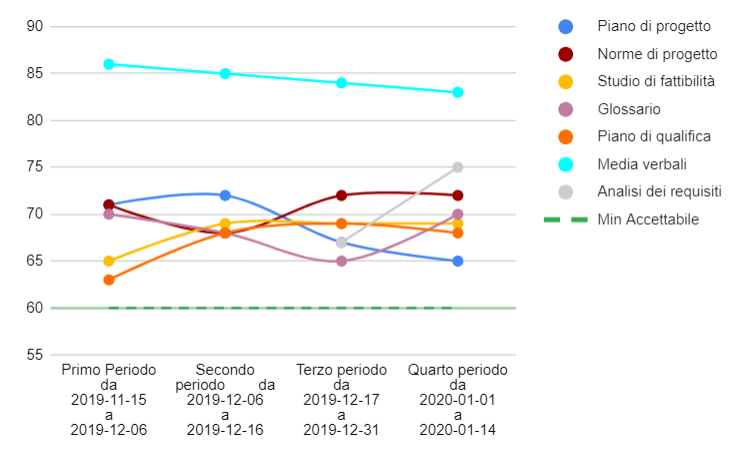
\includegraphics[width=0.8\linewidth]{./res/images/gulpease.png}
	\caption{Grafico periodo/indice di gulpease nel periodo di Analisi dei Requisiti}
	\label{fig:Grafico indice di gulpease periodo di Analisi dei Requisiti}
\end{figure}

\subsubsection{Calcolo ortografia documenti}
E' stato effettuato un controllo di ortografia e di seguito vengono illustrati i risultati ottenuti durante il periodo di Analisi dei requisiti:

\begin{figure}[H]
	\centering
	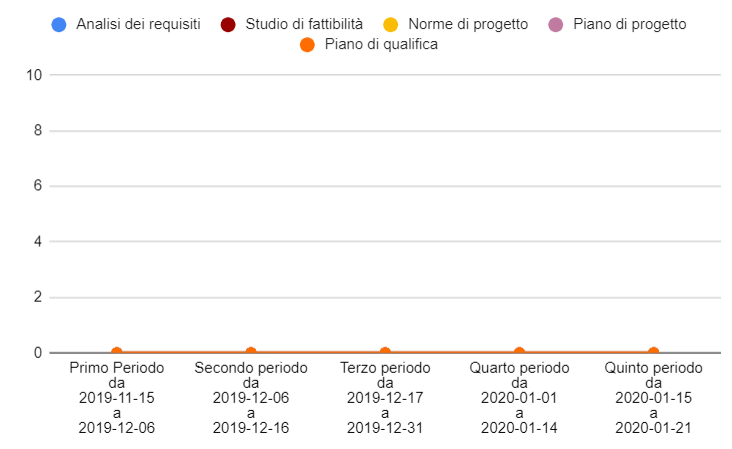
\includegraphics[width=0.8\linewidth]{./res/images/ortografia.png}
	\caption{Grafico periodo/errori ortografici nel periodo di Analisi dei Requisiti}
	\label{fig:Grafico errori ortografici periodo di Analisi dei Requisiti}
\end{figure}